\documentclass[aspectratio=169,10pt]{beamer}
\usepackage{teaching_slides}


\title{Diversion Ratios}
\author{Chris Conlon}
\institute{NYU Stern}
\date{Fall 2026}

\begin{document}

\frame{\titlepage}
\section{What are Diversion Ratios?} 

\begin{frame}{Horizontal Merger Guidelines (2010 rev.)}
\begin{quote}
In some cases, the Agencies may seek to quantify the extent of direct competition between a product sold by one merging firm and a second product sold by the other merging firm by estimating the diversion ratio from the first product to the second product. The diversion ratio is the \alert{fraction of unit sales lost by the first product due to an increase in its price that would be diverted to the second product}. Diversion ratios between products sold by one merging firm and products sold by the other merging firm can be very informative for assessing unilateral price effects, with \alert{higher diversion ratios indicating a greater likelihood of such effects}. Diversion ratios between products sold by merging firms and those sold by \alert{non-merging firms have at most secondary predictive value.}
\end{quote}
\end{frame}

\begin{frame}{This time with equations}
 Raise price of good $j$. People leave. What fraction of leavers switch to $k$?
\begin{eqnarray*}
D_{jk} (p_j,\symbf{p}_{-j})= \frac{\frac{\partial q_k}{\partial p_j}}{\left|\frac{\partial q_j}{\partial p_j} \right|}
\end{eqnarray*}
It's one of the best ways economists have to characterize competition among sellers.
\begin{itemize}
\item High Diversion: Close Substitutes $\rightarrow$ Mergers more likely to increase prices.
\item Very low diversion $\rightarrow$ products may not be in the same market.\\ (ie: Katz \& Shapiro). This is just hypothetical monopolist or SSNIP test.
\item Demand Derivatives NOT elasticities.
\item No equilibrium responses.
\end{itemize}
\end{frame}


\begin{frame}{Nevo (2000) Example}
\begin{center}
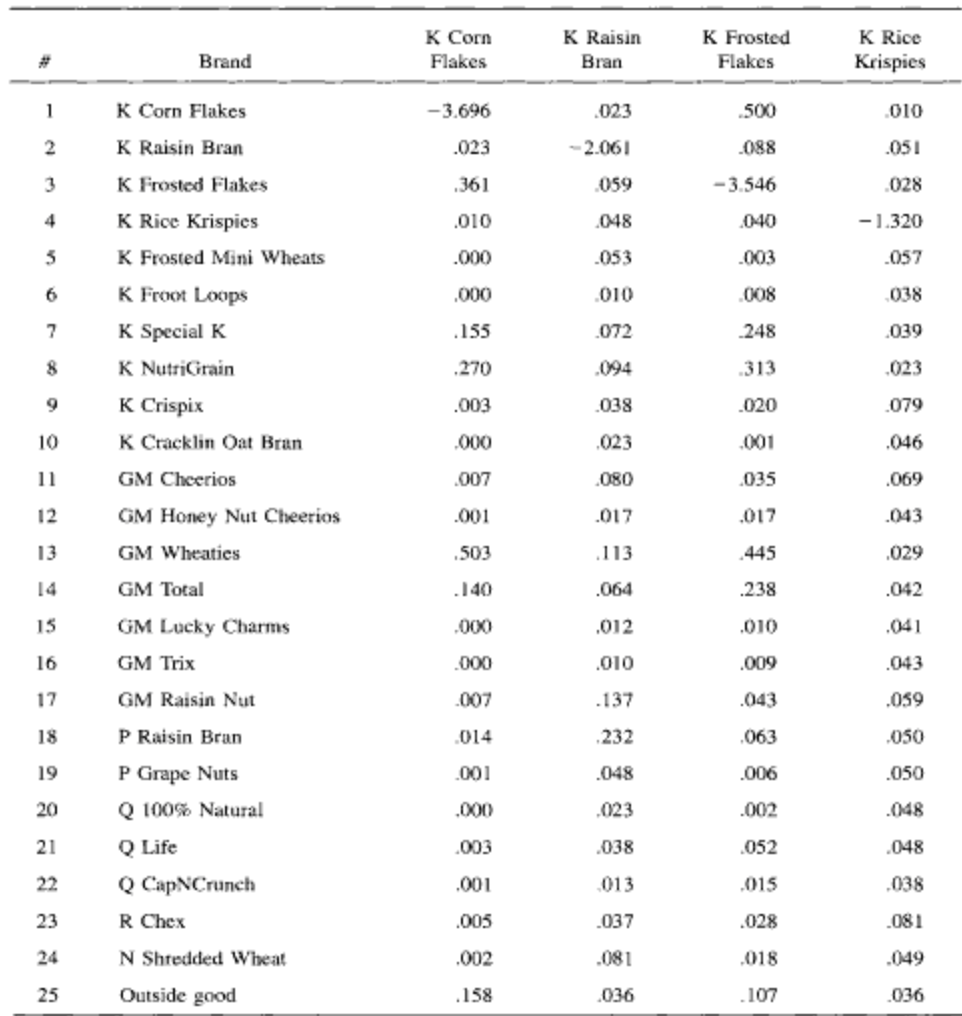
\includegraphics[height=\textheight]{./resources/nevo_elas.png}
\end{center}
\end{frame}



\begin{frame}{Advantages of Diversion}
\begin{itemize}
\item When you were taught elasticities you were taught they were a \alert{unit free} comparison across products, markets, etc.
\item But that is only true of \alert{own elasticities} not cross elasticities.
\item Is $\epsilon_{jt}=.01$ or $\epsilon_{jt}=.03$ a better substitute? We can't tell.
\begin{itemize}
\item You need to take $\epsilon_{jk} \cdot \sigma_k$ to know. If you take $\epsilon_{jk} \cdot \frac{\sigma_k}{p_j} = D_{jk}$ (back at diversion).
\item Because it tells us \alert{fraction of switchers} choosing $k$ we can compare across settings (since share sums to one).
\item ie: diversion ratio $D_{jk} = 0.1$ actually tells me something!
\end{itemize}
\item Whenever you are tempted to report \alert{cross elasticities} report \alert{diversion ratio} instead.
\end{itemize}
\end{frame}


\begin{frame}[plain]
\begin{center}
\scalebox{0.65}{
\begin{tabular}{lrrrrrrr}
\toprule
{} &  Cheerios &  Special K &  Corn Flakes &  Reese's Puffs &  Capt Crunch &  Froot Loops &  Shares \\
\midrule
HN Cheerios         &      5.07 &       4.27 &         3.75 &           5.33 &         3.58 &         3.48 &    2.69 \\
Frosted Flakes      &      2.46 &       2.54 &         4.54 &           4.00 &         5.35 &         7.24 &    2.65 \\
Cheerios            &     -2.46 &       5.91 &         3.13 &           3.19 &         1.36 &         1.77 &    2.10 \\
Honey Bunches       &      2.47 &       2.51 &         2.21 &           2.08 &         1.94 &         1.99 &    1.47 \\
Cinn Toast Crunch   &      3.43 &       2.10 &         1.69 &           3.00 &         1.78 &         1.84 &    1.43 \\
Froot Loops         &      1.26 &       1.19 &         1.64 &           1.69 &         1.82 &        -2.71 &    1.18 \\
Lucky Charms        &      2.18 &       1.64 &         1.57 &           2.99 &         1.59 &         1.58 &    1.14 \\
Frosted Mini-Wheats &      0.36 &       0.50 &         0.74 &           0.68 &         0.87 &         1.27 &    1.01 \\
Corn Flakes         &      2.01 &       2.18 &        -2.64 &           1.31 &         1.24 &         1.52 &    0.98 \\
Rice Krispies       &      1.50 &       1.72 &         1.56 &           0.89 &         0.68 &         1.25 &    0.96 \\
Apple Jacks         &      0.91 &       0.80 &         1.24 &           1.27 &         1.42 &         2.45 &    0.85 \\
Raisin Bran (KEL)   &      0.46 &       0.47 &         0.63 &           0.78 &         0.82 &         1.24 &    0.79 \\
Special K Red Berry &      0.96 &       1.45 &         0.95 &           0.78 &         0.68 &         0.90 &    0.75 \\
Special K           &      2.06 &      -2.66 &         1.18 &           0.71 &         0.44 &         0.58 &    0.74 \\
MG Cheerios         &      1.11 &       0.99 &         0.75 &           0.89 &         0.54 &         0.66 &    0.71 \\
Reese's Puffs       &      1.36 &       0.86 &         0.87 &          -2.70 &         1.08 &         1.01 &    0.69 \\
Life                &      1.15 &       1.12 &         1.05 &           1.02 &         1.72 &         0.89 &    0.68 \\
Cocoa Puffs         &      1.18 &       0.92 &         0.95 &           1.47 &         1.05 &         0.97 &    0.67 \\
Capt Crunch         &      0.63 &       0.58 &         0.88 &           1.21 &        -2.68 &         1.19 &    0.62 \\
Capt Crunch Berry   &      0.68 &       0.61 &         0.83 &           1.15 &         3.29 &         1.00 &    0.58 \\
Corn Pops           &      0.43 &       0.43 &         0.71 &           0.66 &         0.75 &         1.45 &    0.56 \\
Cinn Life           &      0.76 &       0.75 &         0.83 &           0.84 &         1.59 &         0.78 &    0.54 \\
Fruity Pebbles      &      0.61 &       0.59 &         0.71 &           0.71 &         0.75 &         0.77 &    0.44 \\
\bottomrule
\end{tabular}

}
\end{center}
\end{frame}





%\begin{frame}
%\frametitle{Antitrust Policy -- Horizontal Mergers}
%Antitrust authorities use diversion ratios, a la Bertrand, to understand the `unilateral effects' of proposed mergers.
%\begin{itemize}
%\item Unilateral effects: competition between products of the merged firm is reduced because the merged firm internalizes substitution between jointly-owned products.
%\item Unilateral effects can lead to price increases.
%\item Current U.S. merger guidelines:\\
%\indent \textit{\footnotesize Diversion ratios between products [of the merging firms] can be very informative for assessing unilateral price effects.}
%\item Higher diversion between merging products pre-merger $\rightarrow$ greater scope for potential price increases.
%\end{itemize}
%\end{frame}

\section{Where do Diversion Ratios come from?\\ (Stolen from Conlon and Mortimer (2021))}


\begin{frame}{Wald Estimator}
The diversion ratio $D_{jk}(p_j,x) \equiv\frac{\partial q_k}{\partial p_j}(p_j,x)/-\frac{\partial q_j}{\partial p_j}(p_j,x)$ can be obtained as the limit of the Wald estimator where the price increase (or decrease) becomes small, so long as demand slopes \textit{strictly} downwards $\frac{\partial q_j}{\partial p_j} <0$.
\begin{align*}                               
\lim_{p_j' \rightarrow p_j} \frac{q_k(p_j',x) - q_k(p_j,x)}{-(q_j(p_j',x) - q_j(p_j,x))} \rightarrow \frac{\frac{\partial q_k}{\partial p_j}(p_j,x)}{-\frac{\partial q_j}{\partial p_j}(p_j,x)} \equiv D_{jk}(p_j,x)
\end{align*}
\end{frame}

\begin{frame}{Analogue to LATE Theorem Imbens Angrist (1994)}
\begin{theorem}[Conlon Mortimer (2021)]\ \\
\label{prop:late}
Under the following conditions:\\ 
(a) Mutually Exclusive and Exhaustive Discrete Choice: $d_{ij} \in \{0,1\}$ and $\sum_{j \in \calJ} d_{ij}=1$.\\
(b) Exclusion: $u_{ik}(p_j,x)=u_{ik}(p_j',x)$ for all $k \neq j$ and any $(p_j, p_j')$; \\
(c) Monotonicity: $u_{ij}(p_j',x) \leq u_{ij}(p_j,x)$ for all $i$ and any $(p_j' > p_{j})$; and \\
(d) Existence of a first-stage: $\Pr(d_{ij}(p_j,x)=0) \neq \Pr(d_{ij}(p_j',x)=0) $ for $(p_j' > p_{j})$; \\
(e) Random Assignment: $(u_{ij}(p_j,x),u_{ik}(p_j,x)) \perp p_j$. \\
\noindent
then the Wald estimator:
\begin{align*}
 \frac{q_k(p_j',x) - q_k(p_j,x)}{-\left(q_j(p_j',x) - q_j(p_j,x)\right)}=\mathbb{E}[D_{jk,i}(x) | d_{ij}(p_j,x) > d_{ij}(p_j',x)]
\end{align*}
\end{theorem}
\end{frame}

\begin{frame}{Diversion as Treatment Effects}
\begin{description}
\item[Outcome] $Y_i \in \{0,1\}$ denotes the event that consumer $i$ purchases product $k$: $d_{ik}(p_j)=1$.
\item[Treatment] $T_i \in \{0,1\}$ denotes the event that consumer $i$ does \textbf{not} purchase product $j$. In other words $T_i = 0$ implies $d_{ij}(p_j)=1$ and $T_i=1$ implies $d_{ij}(p_j)=0$.
\item[Instrument] $Z_i = p_j$ the price of $j$ induces consumers into not purchasing $j$.
\end{description}
\end{frame}

\begin{frame}{Diversion as MTE}
\footnotesize
What can we learn from a change in $p_j$?
\begin{align*}
\text{Wald}(p_j, p_j',x)
&=\int_{p_j}^{p_j'} D_{jk}(p_s,x) w(p_s) \, \partial \, p_s \mbox{ with }
w(p_s)=\frac{  \frac{\partial q_j(p_s,x)}{\partial p_j} }{\int_{p_j}^{p_j'}  \frac{\partial q_j(p_t,x)}{\partial p_j} \partial p_t} \\
\nonumber &=\int_{p_j}^{p_j'} \int D_{jk,i}(p_s,x)  w_i(p_s,x) \, \partial p_s  \, \partial F_i \quad \mbox{ with } w_i(p_s,x) = \frac{\left| \frac{\partial q_{ij}(p_s,x)}{\partial p_j} \right|}{q_j(p_j,x)- q_j(p_j',x)}\\
&= \int D_{jk,i}(x) \, w_i(z_j,z_j',x)  \, \partial F_i \quad \mbox{ with } w_i(z_j,z_j',x) = \frac{q_{ij}(z_j,x)- q_{ij}(z_j',x) }{q_j(z_j,x)- q_j(z_j',x)}
\end{align*}
\begin{itemize}
\item Individual diversion ratios in logit family are $D_{jk,i} = \frac{\sigma_{ik}}{1-\sigma_{ij}}$ and don't depend on $p_j,z_j$
\item Which individuals respond to $z_j$ or $p_j$ determines the weighting scheme only.
\end{itemize}
\end{frame}

\begin{frame}{Weights}
Again $D_{jk,i} = \frac{\sigma_{ik}}{1-\sigma_{ij}}$ for logit family:\\
\begin{center}
\begin{tabular}{rcc} 
& $w_{i j}(x) \propto$ \\
\midrule second choice data & $\sigma_{i j}(x)$ \\
price change $\frac{\partial}{\partial p_{j}}$ & $\sigma_{i j}(x) \cdot\left(1-\sigma_{i j}(x)\right) \cdot\left|\alpha_{i}\right|$ \\
characteristic change $\frac{\partial}{\partial x_{j}}$ & $\sigma_{i j}(x) \cdot\left(1-\sigma_{i j}(x)\right) \cdot\left|\beta_{i}\right|$ \\
small quality change $\frac{\partial}{\partial \xi_{j}}$ & $\sigma_{i j}(x) \cdot\left(1-\sigma_{i j}(x)\right)$ \\
finite change in $z_j$ & $\sigma_{ij}(z_j') - \sigma_{ij}(z_j)$\\
\midrule
\end{tabular}
\end{center}
\begin{itemize}
\item Normalize so that above weights sum to one $w_{ij}^* = w_{ij}/\int w_{ij} \, d F_i$
\item For plain logit $D_{jk,i} = \frac{\sigma_{k}}{1-\sigma_{j}}$ for all $i$ and weights don't matter!
\end{itemize}
\end{frame}

\begin{frame}{Mixed Logit, Second Choices}
Here we get a really simple decomposition:
\begin{align*}
D_{j \rightarrow k} = \sum_{i \in \mathcal{I}} \underbrace{\frac{\sigma_{ik}}{1-\sigma_{ij}}}_{D_{jk,i}} \cdot \underbrace{\frac{w_i \cdot \sigma_{ij}}{\sigma_{j}}}_{\gamma_{ij}}
\end{align*}
Idea: different interventions change \alert{weights} but not \alert{individual diversion ratios}:
\begin{itemize}
\item \textbf{Individual Diversion Ratios} $D_{jk,i}$ : $\Pr( i \text{ chooses } k \mid \text{ doesn't choose } j)$.

\item \textbf{Weights} $\gamma_{ij}$ : For second choices: $\Pr(\text{Type } i \mid \text{ leaves } j) =\Pr(\text{Type } i \mid \text{ chooses } j)$.\\ For infinitesimal price changes $\gamma_{ij}=\frac{w_i \cdot |\beta_i^p| \cdot \sigma_{ij}(1-\sigma_{ij})}{\sum_{i
 \in \mathcal{I}} w_{i'} \cdot |\beta_i^p| \cdot \sigma_{i'j}\cdot(1-\sigma_{i'j})}$ or finite: $\gamma_{ij}(p_j,p_j')=\frac{\sigma_{ij}(p_j')-\sigma_{ij}(p_j)}{\sigma_{j}(p_j')-\sigma_{j}(p_j)}$.\\
 (Types that are: price sensitive and likely to choose $j$).\\
 But we could do this with anything (not just price!)
\end{itemize}
\end{frame}


\begin{frame}{Application of CM Decomposition: Customer Overlap (Einav, Guido, Klenow, AER:I 2026)}
\small
Panel data (credit cards, cell-phone traces, Nielsen panelists) record $T_i$ purchases per consumer but no second-choice question. Let $q_{ik}$ be $i$'s purchases of $k$, $\sum_k q_{ik} = T_i$, and $\mathcal{C}_j = \{i : q_{ij} \geq 1\}$ the consumers \alert{ever observed buying} $j$ (Starbucks). EGK propose the \alert{customer overlap}:
\begin{align*}
C_{j \rightarrow k}
=\frac{\sum_{i \in \mathcal{C}_j} q_{ik}}{\sum_{i \in \mathcal{C}_j} (T_i - q_{ij})}
= \sum_{i \in \mathcal{C}_j} \underbrace{\frac{\hat{\sigma}_{ik}}{1-\hat{\sigma}_{ij}}}_{\hat{D}_{jk,i}} \cdot \underbrace{\frac{T_i - q_{ij}}{\sum_{i' \in \mathcal{C}_j} (T_{i'}-q_{i'j})}}_{w_i^{\mathcal{C}}}
\qquad \text{with } \hat{\sigma}_{ij} = q_{ij}/T_i.
\end{align*}
\begin{itemize}
    \item Fits the CM decomposition: a weighted average of \alert{individual diversion ratios}, weights $\propto$ non-$j$ purchases.
    \item Two forces pull in opposite directions. \emph{Conditional} on $i \in \mathcal{C}_j$, weight is heaviest on consumers \alert{least} loyal to $j$; \emph{selection} into $\mathcal{C}_j$ favors the \alert{most} loyal (they are the ones observed buying $j$ at all).
    \item How much they cancel depends on panel length $T_i$. Assume mixed logit with persistent $V_{ij}$ and iid $\varepsilon_{ijt}$ across purchase occasions, so $q_{ij} \sim \text{Binomial}(T_i, \sigma_{ij})$ and we can work it out (next slide).
\end{itemize}
\end{frame}


\begin{frame}{What Does Overlap Measure? (Conlon, Mortimer, Sarkis 2026, Appendix)}
\small
Population analogue (type weights $w_i$, per-type panel weight $\overline{w}_i(\sigma_{ij}) \equiv \E\left[T_i \left(1-(1-\sigma_{ij})^{T_i-1}\right) \mid i\right]$):
\begin{align*}
C_{j \rightarrow k} = \frac{\sum_i w_i\, \sigma_{ik}\, \overline{w}_i(\sigma_{ij})}{\sum_i w_i\, (1-\sigma_{ij})\, \overline{w}_i(\sigma_{ij})}
= \sum_i \underbrace{\frac{w_i (1-\sigma_{ij}) \overline{w}_i(\sigma_{ij})}{\sum_{i'} w_{i'} (1-\sigma_{i'j}) \overline{w}_{i'}(\sigma_{i'j})}}_{\gamma_{ij}^{(C)}} \cdot D_{jk,i}
\end{align*}
\vspace{-0.2cm}
\begin{center}
\renewcommand{\arraystretch}{1.2}
\begin{tabular}{lll}
\toprule
Panel length & $\gamma_{ij}^{(C)} \propto$ & $C_{j \rightarrow k}$ equals \\
\midrule
$T_i = 2$ for everyone & $w_i\, \sigma_{ij} (1-\sigma_{ij})$ & \alert{quality diversion} $D^{\xi}_{j \rightarrow k}$ (the $\partial/\partial \xi_j$ row of the weights table), exactly \\
small $\sigma_{ij}$, moderate $T_i$ & $\approx w_i\, \sigma_{ij} (1-\sigma_{ij})$ & $\approx$ quality diversion (degrades for loyal $j$-buyers) \\
$T_i \rightarrow \infty$ & $w_i (1-\sigma_{ij})$ & \alert{IIA logit} $\sigma_k/(1-\sigma_j)$: all heterogeneity gone \\
\bottomrule
\end{tabular}
\end{center}
\begin{itemize}
    \item The longer the panel, the \alert{less} the raw overlap tells you: every type eventually enters $\mathcal{C}_j$ and the selection no longer discriminates.
    \item Regimes assume $T_i$ independent of type; heavy users observed longer tilt the weights by $\E[T_i \mid i]$.
\end{itemize}
\end{frame}


\begin{frame}{A Better Overlap Measure: Odds-Ratio Reweighting (CMS 2026, Appendix)}
\small
Same data $(q_{ij}, q_{ik}, T_i)$. Weight each consumer by their share of $j$'s purchases $q_{ij}/Q_j$ instead of by their non-$j$ purchases (equivalently: reweight EGK by the odds $\hat{\sigma}_{ij}/(1-\hat{\sigma}_{ij})$):
\begin{align*}
A_{j \rightarrow k} = \frac{1}{Q_j} \sum_{i:\, q_{ij} < T_i} \frac{q_{ij}\, q_{ik}}{T_i - q_{ij}}
= \sum_i \underbrace{\frac{\hat{\sigma}_{ik}}{1-\hat{\sigma}_{ij}}}_{\hat{D}_{jk,i}} \cdot \underbrace{\frac{\hat{\sigma}_{ij}}{\sum_{i'} \hat{\sigma}_{i'j}}}_{\hat{\gamma}_{ij}^{\text{second choice}}}, \qquad Q_j = \sum_i q_{ij}.
\end{align*}
\begin{itemize}
    \item These are the empirical \alert{second-choice weights} $\gamma_{ij} = w_i \sigma_{ij}/\sigma_j$ from two slides ago. No conditioning on $\mathcal{C}_j$; consumers with $q_{ij}=0$ or $q_{ij}=T_i$ contribute nothing.
    \item Population limits: $T_i = 2 \Rightarrow$ quality diversion (same as EGK); $T_i \rightarrow \infty \Rightarrow$ \alert{second-choice diversion} $D_{j \rightarrow k}$. It \alert{improves} with panel length rather than collapsing to IIA.
    \item Either version is a legitimate input to the product-space estimator in the next deck, as long as the model-side formula matches (quality vs.\ second-choice weights differ by a factor $(1-\sigma_{ij})$, $\approx 1$ when shares are small).
    \item Caveats: $\hat{\sigma}_{ij}$ is noisy at small $T_i$; assumes a stable environment over the panel (no entry/exit, price changes) and persistent $V_{ij}$ with iid $\varepsilon_{ijt}$.
\end{itemize}
\end{frame}


\begin{frame}{Welfare and WTP: Diversion to the Outside Good}
Recall the worked removal example from the logit lecture: for a member of the logit family, the welfare loss from removing $j$ is $\Delta CS_i = \frac{1}{\alpha_i}\log(1-\sigma_{ij})$. The same object, written in the language of this lecture:
\begin{align*}
WTP_i(j) = \log \left( \frac{\sigma_{i0}(\calJ\setminus j) }{\sigma_{i0}(\calJ) }\right)
=\log \left( 1+\frac{D_{j0,i}\, \sigma_{ij}}{\sigma_{i0}(\calJ) }\right)
=\log \left( 1+\frac{\sigma_{ij}}{1-\sigma_{ij}  }\right)
\approx \frac{\sigma_{ij}}{1-\sigma_{ij} }
\end{align*}
using $\sigma_{i0}(\calJ\setminus j) = \sigma_{i0}(\calJ) + D_{j0,i} \cdot \sigma_{ij}$ and $D_{j0,i} = \frac{\sigma_{i0}}{1-\sigma_{ij}}$.
\begin{itemize}
\item Welfare and willingness to pay are mostly about \alert{diversion to the outside good} (HW2).
\item Individual willingness to pay is exclusively about \alert{own share}, not the presence of close substitutes. Is this a good property or not?
\item This is the $WTP_i(j)$ that drives the hospital-network literature (Capps, Dranove, Satterthwaite 2003), coming up in the Health IO lecture.
\end{itemize}
\end{frame}

\begin{frame}{Practical Tips: Checklist}
\begin{itemize}
\item How much diversion to outside good?
\item What are top substitutes by diversion? How much do they get?
\item Do identities of best substitutes differ across products?
\item How much diversion goes to own products vs. competitors?
\item For mergers, what would \alert{divestiture} candidates be?
\end{itemize}
\end{frame}




\end{document}